\documentclass{article}
\usepackage[utf8]{inputenc}

\title{Домашнее задание № 5}
\author{Иван Нечепуренко }
\date{September 2018}

\usepackage{natbib}
\usepackage{graphicx}
\usepackage{amsmath,amsfonts,amssymb,amsthm,mathtools} % AMS
\usepackage[english,russian]{babel}	% локализация и переносы

%%% Работа с картинками
\usepackage{graphicx}  % Для вставки рисунков
\graphicspath{{images/}}  % папки с картинками
\setlength\fboxsep{3pt} % Отступ рамки \fbox{} от рисунка
\setlength\fboxrule{1pt} % Толщина линий рамки \fbox{}
\usepackage{wrapfig} % Обтекание рисунков и таблиц текстом

\begin{document}

\maketitle

Для начала пронумеруем все условия эксремума из теоремы Каруша-Куна-Такера, чтобы затем быстро на них ссылаться:
\begin{align*}
&1) g_i(x^ *) = 0, i = 1, . . . , m \\
&2) h_j(x^*) \leq 0, j = 1, . . . , p \\
&3) \mu^*_j \geq 0, j = 1, . . . , p \\
&4) \mu^*_j h_j(x^*) = 0, j = 1, . . . , p \\
&5) \Delta_x L(x^*, \lambda^*, \mu^*) = 0 
\end{align*}

\section{Задача 1}
Обозначим (*) - утверждение об невырожденности матриц. Выведем следующие импликации:

(*) $\Longrightarrow$(a) Предположим противное. $\exists x \neq \overline{0}: Ax = 0, Px = 0$. Тогда составим вектор $(x, \overline{0})$ размерности $n + m$, не являющийся нулевым. Но при этом, если его умножить на блочную матрицу, получится нулевой вектор. Это противоречит невырожденности матрицы.

(a)  $\Longrightarrow$ (d) Идем от противного. Достаточно взять $Q = E_m$. Тогда $\forall x \neq 0: x^T(P + A^TA)x \geq 0$. Равенство достигается при $x^TPx = 0$, $(Ax)^T(Ax) = 0$. Отсюда следует, что $Ax = 0$, но, из условия а) следует, что $Px \neq 0$. Но мы знаем, что из положительно полуопределенной матрицы можно вычислить симметричный корень. Пишем $x^TPx = x^T \sqrt{P}^T \sqrt{P} x = (\sqrt{P} x)^T(\sqrt{P} x) = 0 \longrightarrow \sqrt{P} x = 0$. Но тогда $Px = \sqrt{P}^T\sqrt{P} x = 0$. Мы пришли к противоречию.

(d)  $\Longrightarrow$ (c) Рассмотрим отображение, порожденное $A$. Ранг $A$ - m, размерность образа - такая же. Но тогда размерность ядра - $ n - m$. Тогда таков размер образа от отображения, порожденного $F$, и это значение совпадает с минималным размером $F$. Отсюда $F$ - невырожденная(ну, в смысле, как задающая отображение с нулевым ядром) матрица, $Fx = 0 \longrightarrow x = 0$. Достаточно было даже просто заметить, что F - это матрица, составленная из векторов фундаментальной системы решений, которые по определению независимы. Также по определению $F$ $\forall x AFx = 0$. Но тогда можно рассмотреть сужение d) на образ $F$. Выходит $ \forall x x^T(F^TPF + F^TA^TQAF)x = x^T(F^TPF)x  \geq 0$, равенство достигается только при $ Fx = 0$, т.е. $x = 0$. Но это и есть условие (c)

(c)  $\Longrightarrow$ (b) $Ax = 0, x \neq 0 \longrightarrow \exists y \neq 0, x = Fy$( $F$ - система фундаментальных решений). Тогда $x^TPx = y^TF^TPFy > 0$, при $y \neq 0$

(b) $\Longrightarrow$ (*)
Приравняв блочную матрицу нулю, рассмотрим некоторое решение уравнения $(x, \lambda)$
$$ Ax = 0 \longrightarrow x^TA^T = 0 \longrightarrow x^TA^T\lambda = 0$$
$$ Px + A^T \lambda = 0 \longrightarrow x^TPx + x^TA^T \lambda = 0 \longrightarrow x^TPx = 0 \longrightarrow x = 0$$
Но тогда получается $Px = 0$. $A^T \lambda = 0$. Система - ранга $p$ с $p$ переменными, а это значит, что она невырождена, $\lambda = 0$. $(x, \lambda ) = 0$, а из этого следует, что блочная матрица(обозначим $B$) - невырождена.

\section{Задача 2}
а) Записываем Лагранжиан, приравниваем нулю:
$$ 2x + \mu(x - 2) + \mu(x - 4) = 0$$
Также выпишем условие типа 4):
$$ \mu(x - 2)(x - 4) = 0$$
Из него выходит, что нам достаточно рассмореть случаи $\mu = 0$, $x = 2$, $x = 4$. Тогда получаются возможные пары $(\mu, x)$: $(0, 0)$, $(2, 2)$, $(-4, 4)$. Первая пара не подходит по условию 2), последняя - по условию 3), вторая удовлетворяе всем условиям и являеся точкой мнимума (минимум - 5), так как задача выпуклая. 

б)

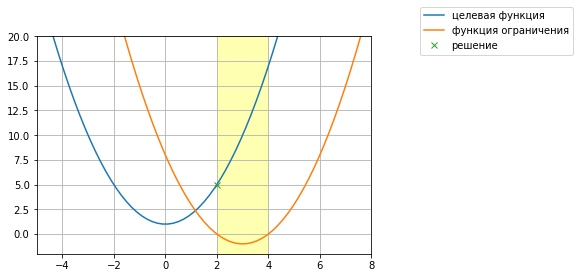
\includegraphics[scale=0.7]{pic1.jpg}

в)

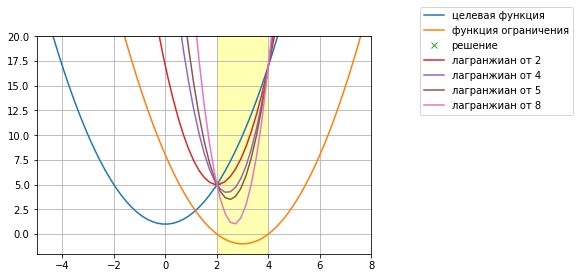
\includegraphics[scale=0.7]{pic2.png}

Видим, что "низушки" парабол действительно находятся не выше точки $(2, 5)$

г) Перепишем Лагранжиан:
$$L(x, \mu) = (1 + \mu)x^2 -6\mu x + 8\mu + 1$$
$\mu \geq 0$, отсюда $1 + \mu > 0$, и минимум приходится на $\displaystyle x = -\frac{b}{2a} = \frac{3\mu}{\mu +  1}$. Подставив это в Лагранжиан, получаем, что нужно максимизировать 
$$ \frac{-\mu^2 + 9\mu + 1}{\mu + 1}$$
Максимум достигается при $\mu = 2 > 0$, и соответствующее значение Лагранжиана - $5$, является точной нижней оценкой $x^2 + 1$, а значит, задача сильно двойственна.

\section{Задача 4} 
На семинаре обсуждалось то, что по условию Сейлера квадратичное программирование с квадратичными(как частный случай - линейными) ограничениями, явлается сильно двойственной. Особенно хорошо это ясно из того, что множество, задаваемое ограничениями, не просто выпуклое, но афинное, а огр-й типа неравенств нет.

Начнем с прямой задачи. Заметим, что минимум $\displaystyle \frac{1}{2} ||Ax -b||^2_2$ и $\displaystyle ||Ax -b||^2_2$ достигается на одних и тех же $x$, а это значит, что нам можно минимизировать и первое выражение. Так и поступим.
$$L(x, \lambda) = \Delta (\frac{1}{2}(Ax -b)^T(Ax - b) + \lambda^T (Gx - h)) $$
$ \displaystyle
\frac{\partial}{\partial x} (\frac{1}{2}x^TA^TAx -x^TA^Tb + \frac{1}{2}b^Tb + \lambda^T (Gx - h)) =
\frac{\partial}{\partial x} (\frac{1}{2}x^TA^TAx -x^TA^Tb + \frac{1}{2}b^Tb + x^TG^T\lambda - \lambda^Th) =
A^TAx - A^Tb + G^T\lambda = 0
$

$
 \displaystyle \frac{\partial}{\partial \lambda} L(x, \lambda) = Gx - h = 0 
$

Теперь запишем получившуюся систему,которую мы теперь должны решить:
$$A^TAx + G^T\lambda =  A^Tb$$
$$Gx = h$$
Нам нужно определиться, какие матрицы являются невырожденными. Рассмотрим $A^TA$. $x^TA^TAx = (Ax)^T(Ax) \geq 0$, т. е. $A^TA$ - неотрицательно определенная квадатичная форма, и её ядро совпадает с ядром соответствующего отображения. Но из соображений ранга оно - нулевое. А это значит, что $A^TA$ - невырожденная матрица. По тем же соображениям невырождена матрица $GG^T$. Тогда задачу можно решать "в лоб":
$$ x + (A^TA)^{-1}G^T\lambda - (A^TA)^{-1}A^Tb = 0$$
$$ h + G(A^TA)^{-1}G^T\lambda - G(A^TA)^{-1}A^Tb = 0$$
$$ G(A^TA)^{-1}G^T\lambda = G(A^TA)^{-1}A^Tb - h$$
$G^T$ - отображение с ненулевым ядром, $(A^TA)^{-1}$ - положительно определенная матрица. Но отсюда $G(A^TA)^{-1}G^T$ - положительно определенная, и, следовательно, невырожденная матрица.
$$ \lambda = (G(A^TA)^{-1}G^T)^{-1}(G(A^TA)^{-1}A^Tb - h)$$
$$ x = (A^TA)^{-1}(A^Tb - G^T\lambda) = (A^TA)^{-1}(A^Tb - G^T(G(A^TA)^{-1}G^T)^{-1}(G(A^TA)^{-1}A^Tb - h))$$
Худо-бедно $x$ получили, очевидных упрощений не видно.

Переходим к двойственной задаче. Ища минимум Лагранжиана по $x$, мы получаем первое условие(задача выпуклая):
$$ x = (A^TA)^{-1}(A^Tb - G^T\lambda)$$
Т. к. при фиксированном $\lambda$ Лагранжиан - выпуклая ф-ция, эта точка - и есть точка минимума 
Лагранжиана. Ищем его значение в ней: 
$$x^T = (b^TA - \lambda^TG)(A^TA)^{-T} $$
$$x^T = (b^TA - \lambda^TG)(A^TA)^{-1} \longleftarrow (A^TA)^T = A^TA$$
$$x^TA^TAX = (b^TA - \lambda^TG)(A^TA)^{-1} A^TA (A^TA)^{-1}(A^Tb - G^T\lambda) $$
$$x^TA^TAX = (b^TA - \lambda^TG)(A^TA)^{-1} (A^Tb - G^T\lambda) $$
$$x^TA^TAX = (b^TA - \lambda^TG)(A^TA)^{-1} (A^Tb - G^T\lambda) $$ 
$$ x^TA\lambda = (b^TA - \lambda^TG)(A^TA)^{-1} A \lambda$$
И прочая, прочая... Если в конце все подставить в исходное выражение, мы получаем, что задача вогнутая(ну, это всегда так по построению двойственной задачи), в максимуме производная $g(\lambda)$ равняется 0-лю, при выражении из этого(вроде как) получаем $\lambda = (G(A^TA)^{-1}G^T)^{-1}(G(A^TA)^{-1}A^Tb - h)$. Но это значение из прямой задачи, а значит, как и предсказывалось, имеет место сильная двойственность.
\end{document}